\documentclass[a4paper,10pt,oneside,openany]{memoir}

% Aesthetics
\chapterstyle{hangnum}
\renewcommand\contentsname{Table of Contents}

% Set language
\usepackage[british]{babel}

% bibliography
\usepackage[numbers]{natbib}

% Packages
\usepackage{xcolor}
\usepackage[T1]{fontenc}
\usepackage[utf8]{inputenc} % unicode support
\usepackage{tocbibind}
\usepackage{graphicx}
\graphicspath{ {figures/} }
\usepackage{pdfpages} % to import the front page
\usepackage{import}
\usepackage[justification=centering]{caption}% or e.g. [format=hang]
\usepackage{verbatim}
\usepackage{amsmath}

\usepackage{geometry} %% Alter margins on pages

\usepackage{adjustbox}

\usepackage{caption}
\usepackage{subcaption}
\usepackage{tabularx}
\usepackage{color}

% Set margin 
\setlrmarginsandblock{4.5cm}{4.5cm}{*}
\setulmarginsandblock{4.5cm}{*}{1}
\checkandfixthelayout 

% To list code blocks in latex
\usepackage{lstautogobble}
\usepackage{listings}
\lstset{
	language=C,                % choose the language of the code
%	numbers=left,                   % where to put the line-numbers
	stepnumber=1,                   % the step between two line-numbers.        
%	numbersep=5pt,                  % how far the line-numbers are from the code
	backgroundcolor=\color{white},  % choose the background color. You must add \usepackage{color}
	showspaces=false,               % show spaces adding particular underscores
	showstringspaces=false,         % underline spaces within strings
	showtabs=false,                 % show tabs within strings adding particular underscores
	tabsize=2,                      % sets default tabsize to 2 spaces
	captionpos=b,                   % sets the caption-position to bottom
	breaklines=true,                % sets automatic line breaking
	breakatwhitespace=true,         % sets if automatic breaks should only happen at whitespace
%	title=\lstname,                 % show the filename of files included with \lstinputlisting;
	autogobble=true
}

\lstdefinestyle{ttt}{
    basicstyle=\ttfamily,
  %columns=fullflexible,
    mathescape=true,
    literate={->}{$\rightarrow $}{1}
  }

\lstdefinestyle{csv}{
	xleftmargin=-2.5cm,
	xrightmargin=-2.5cm,
	belowskip=0pt,
	basicstyle=\scriptsize,
	stringstyle=\scriptsize,
	fontadjust=true}
% xml listings
\lstdefinestyle{XML}{ 
	columns=fullflexible, 
	basicstyle=\rmfamily, 
	commentstyle=\ttfamily\itshape\color{green!50!black}, 
	morestring=[s]{"}{"}, 
	morecomment=[s]{?}{?}, 
	morecomment=[s]{!--}{--}, 
	morecomment=[s]{!DOCTYPE}{]}, 
	moredelim=[s][\color{black}]{>}{<}, 
	moredelim=[s][\bfseries\color{black}]{\ }{=}, 
	stringstyle=\color{blue}, 
	identifierstyle=\bfseries\color{violet} 
}


%%%%%%%%%%%%%%%
% json listings starts
%%%%%%%%%%%%%%%%
\newcommand\JSONnumbervaluestyle{\color{blue}}
\newcommand\JSONstringvaluestyle{\color{red}}

% switch used as state variable
\newif\ifcolonfoundonthisline

\makeatletter

\lstdefinestyle{json}
{
	showstringspaces    = false,
	keywords            = {false,true},
	alsoletter          = 0123456789.,
	morestring          = [s]{"}{"},
	stringstyle         = \ifcolonfoundonthisline\JSONstringvaluestyle\fi,
	MoreSelectCharTable =%
	\lst@DefSaveDef{`:}\colon@json{\processColon@json},
	basicstyle          = \ttfamily,
	keywordstyle        = \ttfamily\bfseries,
}

% flip the switch if a colon is found in Pmode
\newcommand\processColon@json{%
	\colon@json%
	\ifnum\lst@mode=\lst@Pmode%
	\global\colonfoundonthislinetrue%
	\fi
}

\lst@AddToHook{Output}{%
	\ifcolonfoundonthisline%
	\ifnum\lst@mode=\lst@Pmode%
	\def\lst@thestyle{\JSONnumbervaluestyle}%
	\fi
	\fi
	%override by keyword style if a keyword is detected!
	\lsthk@DetectKeywords% 
}

% reset the switch at the end of line
\lst@AddToHook{EOL}%
{\global\colonfoundonthislinefalse}

\makeatother

%%%%%%%%%%%%%%%
% json listings ends
%%%%%%%%%%%%%%%%

\usepackage{float}
\usepackage[hidelinks]{hyperref}


% glossaries
\usepackage{glossaries}
\newacronym{mad}{MAD}{Median Absolute Deviation} % list of glossaries in a separate file

\newcounter{quote}

\newcommand\citea[1]{%
	(\citeauthor{#1},~\citeyear{#1})}

\newcommand\citeap[2]{%
	    \ifx&#1&%
	    % #1 is empty
	    (\citeauthor{#2},~\citeyear{#2})
	    \else
	    % #1 is nonempty
	    (\citeauthor{#2},~\citeyear{#2}:#1)%%
	    \fi
}
	
% enquote some text
\newcommand{\q}[1]{``#1''}
\newcommand{\qe}[1]{``\emph{#1}''}

% Commands
% Horizontal lines used for the Front Page Title
\newcommand{\HRule}{\rule{\linewidth}{0.5mm}}

\begin{document}

%\frontmatter{}

% Standard Frontpage
%TODO INCLUDE STANDARD FRONTPAGE
%\includepdf[pages={1}]{standardfrontpage2.pdf}

%TODO INCLUDE NORMAL FRONTPAGE
\begin{center}
  \thispagestyle{empty}

  % Header text
  \textsc{\LARGE IT University of Copenhagen}\\[0.5cm]
  \textsc{\Large  (Thesis)}\\[2cm]

  % Title in box
  \HRule\\[0.4cm]
  {\huge \bfseries Untitled Thesis Project \\ [0.4cm]}
  \HRule\\[3cm]

  % Author and supervisor
  \begin{tabular}{lr}
  	\textit{Authors:} \\
    Ans Uddin                     & \texttt{anud@itu.dk} \\
    \\
    \\
    \\
    \textit{Supervisor:}\\
    Willard Rafnsson \\
    \\
    \textit{Co-supervisor:}\\
    Carsten Schürmann\\
  \end{tabular}

  \vfill
  {\large February, 2018}
\end{center}



\pagenumbering{roman}
\setcounter{secnumdepth}{-1}
\frontmatter{}

\chapter{Abstract}

The thesis is a case study of secure implementation using the Information-Flow Control tool Paragon on top of the Matrix protocol. The implementation is a prototype inspired by Danish patient journals systems which requires end-to-end security. End-to-end security is the guarantee of confidentiality and integrity throughout the system. Matrix is a secure communication protocol that ensures confidentiality and integrity of information through end-to-end encryption. However encryption provides no such guarantees once the information is decrypted at the endpoints. Information-Flow Control is such a mechanism that can ensure confidentiality and integrity at the endpoints by enforcing security policies. Paragon is a Java based programming language with the ability to define and enforce security policies.

The thesis contributes with a interface between Paragon and Matrix allowing implementations with end-to-end security on top of Matrix.





\chapter{Acknowledgements}
\input{tex/Acknowledgements}

\pagebreak


\setcounter{tocdepth}{3}
\setcounter{secnumdepth}{3}

\tableofcontents*
\chapter*{List of Tables}
\chapter*{List of Figures}








\mainmatter{}

\pagenumbering{arabic}
\chapter{Introduction}\label{intro}
\section{Data privacy and protection}

With GDPR becoming effective in 2018 the focus on data privacy is at its peak. 
Privacy violation is when sensitive data is exposed to unauthorized actors\cite{cwe}. OWASP top ten ranks \emph{sensitive data exposure} as 3rd biggest security threat\cite{owasp}. 

Recent cases of data leakage has put more attention on data privacy and protection. Some cases are due to poor security measures and could arguably have been prevented. Examples of cases are:

\begin{itemize}
	\item The infamous Facebook - Cambridge Analytica scandal. Third parties were able to collect data through Facebook Login API.
	\item Google Plus leak. 500.000 users private data was exposed to third parties through APIs\cite{googleplus}.
	\item Medicaid leak. A medical assistant had accessed patients' health records and exchanged mails with another employee containing the patients' private data\cite{medicaid}.  
\end{itemize}


%https://www.nytimes.com/2018/10/08/technology/google-plus-security-disclosure.html
%https://www.seattletimes.com/seattle-news/health/91000-state-medicaid-clients-warned-of-data-breach/

The cases above failed to achieve end-to-end security and the improper handling of sensitive data could have been prevented with appropriate security policies and enforcement technique that enforces these policies.

There is more awareness on how applications deal with data. This add extra concern to the programmer and the application about how sensitive data is handled and protected.  

The well-known security enforcement techniques like access controls, firewalls and encryption are inadequate alone and does not ensure end-to-end security\cite{Sabelfeld2003}.




%https://cwe.mitre.org/data/definitions/359.html


%OWASP top ten A3 sensitive data exposure


\section{Information Flow Control} % ikke teknisk. hvilke problemer løser ifc -> lave eksempeler med kode

There exist useful security enforcement mechanisms for protecting confidential information such as firewalls, encryption and access control. However, these mechanisms each have their drawbacks.

\begin{itemize}
	\item \emph{Access} control prevents unauthorized access to information but once access is granted there is no guarantee how that confidential information is handled.
	\item \emph{Firewall} limits communication from the outside hence isolate and protect information. Yet the firewall have no way of telling if the communication going through violates confidentiality.
	\item \emph{Encryption} secures information on a channel with only the endpoints being able to access that information. However there is no assurance that once the data is decrypted that the confidentiality of that information is ensured.
\end{itemize}

The mechanisms mentioned above all have in common that they lack control of how the information flows. Information-flow security aims at protecting confidentiality and integrity of information by enforcing security policies. Information-Flow Control allows the programmer to define and enforce policies in a language-based way\cite{Sabelfeld2003}. 



\section{Matrix}\label{matrix:intro}
Matrix is an open standard protocol for messaging over HTTP and synchronizing data. Matrix provides secure real-time communication over a decentralized federated network. Matrix secures data by providing end-to-end encryption.

Matrix cover use cases such as instant messaging, VoIP, Internet of Things communication and is generally applicable anywhere for subscribing and publishing data over standard HTTP API.
 
The fragmentation of IP communication is the problem Matrix essentially wants to solve. Making calls and messages between users needless of which app they use. However they define their longer term goal as \emph{"to act as a generic HTTP messaging and data synchronisation protocol for the whole web"}\cite{matrixfaq}.



%https://matrix.org/docs/guides/faq
%However in the presence of end-to-end encryption, apps can still leak through their application logic; a content-filtering chat bot running at the receiving end of an end-to-end encrypted connection can leak anything it receives from this connection. 



\section{The case study} % Challenges 

The goal of the case study is to make secure implementation of a prototype using Information-Flow Control. The case study will use Matrix as the communication channel and strengthen the security at the endpoints using IFC.

\subsection{Journal system}
The prototype implements a journal system and is loosely based on the Danish E-journal system.

%https://journalofethics.ama-assn.org/article/electronic-health-records-privacy-confidentiality-and-security/2012-09
Medical privacy is a well-known issue\cite{Rahim2013}. Sensitive data about patients needs to be handled carefully. In Denmark patients have access to their medical records through E-journal\cite{ejournal}. A patient's journal on E-journal is available for up to 90.000 different medical employees\cite{JP90000}. 

There are clear policies about who and under what conditions should access a journal. It is legally required that an employee accessing the journal must have the patient in care and that the lookup must be relevant for the employee. Safety measures have been applied through logging and audit trails with random sampling checks however they do not prevent access to journals. Any medical employee can access the patient journal and even if prevention mechanism were established there would be no limitation to what a medical employee could see once access was granted \cite{adgang}\cite{kontrol}. 

%Example of a being referred to a physician. A physician can access the patient journal but can see full history of the patient sessions. If the patient had psychiatric treatment it would be of no relevance to that medical employee. 

%https://www.sundhed.dk/borger/service/om-sundheddk/om-portalen/datasikkerhed/andres-dataadgang/adgang-til-sundhedsdata/

The mechanisms in the current journal system might restrain malicious intend. However it does not guarantee prevention of unintentional access or disclosure of information\cite{Harman2012}. 
What is missing is the enforcement of secure information flow policies. Unintentional access or disclosure of information can be prevented by enforcing policies that define secure information flow.

The prototype will model a simplified scenario of hospitals with different actors accessing a patient journal. The bulk of information on the journal system is extracted from newspaper articles hence there is a high uncertainty of how the system really works. Therefore many assumptions are made about the current system when programming the prototype.


%https://journalofethics.ama-assn.org/article/electronic-health-records-privacy-confidentiality-and-security/2012-09


%https://cwe.mitre.org/data/definitions/359.html

%https://www.version2.dk/artikel/e-journals-systemadministrator-vi-vaerner-patienternes-privatliv-1059692
%Vi kan ikke garantere, at alle bliver opdaget, men borgerne kan se i 'Min log', hvem der har været inde og se på deres data. Derudover laves der en auditering, hvor ca. fire procent af alle opslag undersøges, og der verificeres, om der har været en behandlerrelation.
%Loggen på sundhed.dk viser kun de tilgange til journalen der har været via netop sundhed.dk. Læger, apoteker m.m. har nemlig også en adgang til sundhed.dk hvor de kan slå folk op - og det bliver logget. Men loggen i sundhed.dk viser IKKE de opslag der sker i alle de andre systemer i sundhedsvæsenet, f.eks. patientjournal-systemerne. 
%https://www.version2.dk/artikel/90000-ansatte-har-adgang-til-patientjournaler-stikproever-er-eneste-kontrol-58628
%https://jyllands-posten.dk/indland/ECE6715461/op-imod-90000-ansatte-kan-kigge-i-din-journal/
%https://www.dr.dk/nyheder/regionale/sjaelland/it-systemer-snakker-ikke-godt-nok-sammen-risikerer-gaa-ud-over

\subsection{Scope} 
%Selvom jeg ikke kiggr på fx trafic analysis så er det vigtigt at nævne og påpege det ikkeer noget jeg løser.

% Clarify at the exam what is meant by the Matrix security model described in the project proposal 

% The goal of the thesis is not to reimplement Matrix using IFC tools. It is to use Matrix and analyze the security model and see what security guarentees and how we can improve security for the system that uses Matrix. 
The objective of the project is to do a secure implementation of the prototype described above. Secure exchange of patient journal is ensured using Matrix and the endpoints are secured using IFC.

A successful project is one that fulfills these criteria: 

\begin{itemize}
	\item Evaluation of Matrix security model
	\item Survey of IFC tools and selection of tool.
	\item Implement a prototype distributed system running on Matrix, using the chosen tools
	\item Demonstrate increased security guarantee with Matrix and IFC
\end{itemize}   


\subsection{Why Matrix?}
In the Digital Strategy 2016-2020 the Danish Agency of Digitisation defines initiative 7.2 as \emph{"Common standards for secure exchange of information"}. The large number of software systems in the Danish public sector has created a need for an uniform way of exchanging data across different application in a secure manner\cite{TheGovernment2016}. 

The initiative has similarities to the issue Matrix is trying to solve with fragmented IP communication. With Matrix security guarantees and their long term goal as a generic HTTP messaging protocol there is a strong case for using Matrix as a communication channel in this case study.


%Matrix gives security guarantees in term of end-to-end encryption and makes data exchange secure; however the end-points are still vulnerable. By using Matrix as the communication channel it gives gives a stronger security guarantee and adds complexity to the solution being developed using IFC tools. 
 
\section{Method}
 
 \section{Threat model}
 %adversary model
 The threat model is defined in the context of confidentiality and integrity.
 \begin{itemize}
 	\item The adversary has the ability to observe information sent over the network.
 	\item The adversary can generate input to the system .
 	\item The adversary can observe public output.   
 \end{itemize}
 
 % Dolev-yao model
 
 
 
\section{Contribution} %end-to-end security

The contributions to the field are the findings of secure implementation using Paragon and how they compare to similar findings from secure implementation with JIF.

The thesis also contributes with the interface created between Paragon and Matrix making it possible to develop other secure applications on top of secure communication channel Matrix provides. 

 
 
\section{Structure of thesis} % her kan nævnes den antagelse gøres 

Chapter \ref{background} sets the foundation for the thesis and introduces relevant information and background. Chapters \ref{analysis} analyzes the Matrix security model and survey IFC tools. Chapter \ref{design} goes in depth with design of the solution. The results are then presented and discussed in Chapter \ref{results}. The thesis is wrapped up in the conclusion section Chapter 6. 
 
\section{Summary}
There is more awareness on how applications deal with data. This add extra concern to the programmer and the application about how sensitive data is handled and protected. Encryption is an obvious way of ensuring confidentiality; Matrix is a tool that provides end-to-end encryption. However there is no guarantee of encryption of the data is decrypted. Information flow control is such mechanism that enforces security policies throughout the system.



\chapter{Background}\label{background}

This chapter builds the foundation for the thesis introducing relevant concepts and disciplines for the thesis. 


Section \ref{evaluationofmatrix} provides an evaluation of the Matrix security model. The security model is evaluated in the context of a secure messaging system.  
The paper \emph{SoK: Secure Messaging} describes a evaluation framework for evaluating secure messaging systems. They define several security properties related to such systems \cite{sok} which will be presented.


All secure messaging systems with end-to-end encryption are based on the Double Ratchet algorithm from the Signal Protocol which will also be described.


Finally the architecture of Matrix and concepts related to Information-Flow Control will be introduced.

\section{Information security}

Information security is the discipline of protecting information. The key principles in information security are expressed through the CIA model. For a system to be secure these principles should be guaranteed \cite{michael2012}.

\begin{figure}[H]
	\centering
	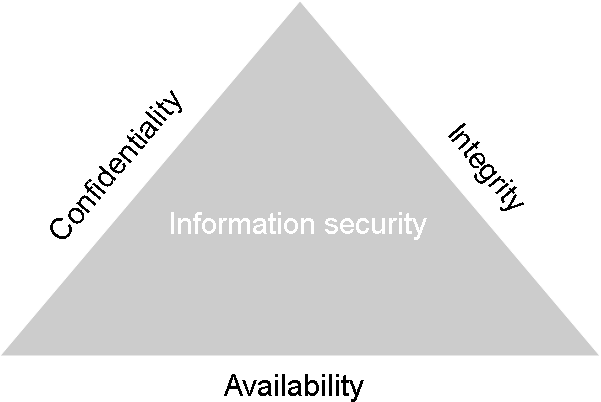
\includegraphics[width=10cm]{figures/cia.png}
	\caption{CIA triad}
	\label{fig:CIA triad}
\end{figure}


\subparagraph{Confidentiality}
Confidentiality is keeping information secret from unauthorized people. This is a major goal in information security. Encryption and access control are common ways of ensuring confidentiality \cite{michael2012}.

In a secure messaging system confidentiality would be guaranteed if the message being sent is only readable by the recipient and no one else \cite{sok}.

\subparagraph{Integrity}
Integrity is providing that information is unaltered and can only be changed by authorized people. If information is intercepted and changed during transit it would be a violation of integrity \cite{michael2012}.  
More specifically for a secure messaging it would mean that no altered message is accepted by the recipient \cite{sok}.

\subparagraph{Availability}
Making sure that information is accessible to authorized people is the goal of availability. Denial of Service attack \footnote{https://en.wikipedia.org/wiki/Denial-of-service\_attack} are common attacks targeting availability. 

Availability is generally more related to the system being available where the information itself plays a minor role \cite{michael2012}.
\\
\\
Depending on the type of system other properties must be satisfied as well. 


\subsection{Security properties}
The goal in a secure messaging system is to protect the messages being sent. The following properties are related to protecting messages.


\subparagraph{Authentication}
When a message is received the participant can verify that the message was sent from the actual sender. Furthermore a participant will receive evidence from a participant in a conversation that hey hold a known long-term secret. 



\subparagraph{Perfect Forward Secrecy}
If all keys are compromised than the decryption of any previously sent message should not be possible. Hence all previous messages would be secure however all future messages would be insecure 

\begin{figure}[H]
	\centering
	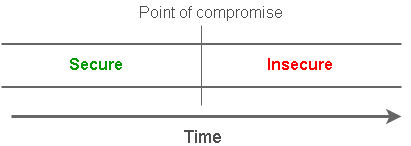
\includegraphics[width=10cm]{figures/forwardsecrecy.png}
	\caption{Forward secrecy}
	\label{fig:forward}
\end{figure}

\subparagraph{Backward secrecy}
If all keys are compromised than the decryption of \emph{future} messages should be possible. This property also goes by the names \emph{future secrecy} and \emph{post compromise security}. 

\begin{figure}[H]
	\centering
	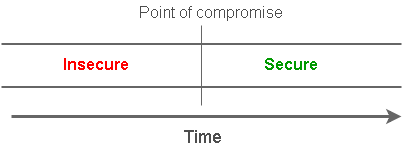
\includegraphics[width=10cm]{figures/backwardsecrecy.png}
	\caption{Backward secrecy}
	\label{fig:backward}
\end{figure}


\subsubsection{Other security properties}


\subparagraph{Participant Consistency} 
Whenever a message is accepted by a participant all participants are guaranteed to have identical view of the participant list.

\subparagraph{Destination Validation}
When a participant receives a message it can be verified that the participant was the intended recipient.

\subparagraph{Anonymity Preserving} 
The anonymity of the participants should be preserved and not linking any key identifiers.

\subparagraph{Speaker Consistency} 
There is consensus among the participants on the sequence of messages they receive by each participant. There might be a mechanism for checking consistency whenever a message is sent or after it has been received.

\subparagraph{Causality Preserving}
Messages must not be displayed before the message that originally precedes it has been displayed.

\subparagraph{Global Transcript} 
A global order where all messages are viewed in the same order for all participants.

\subparagraph{Deniability}
Deniability is a property where other participants cannot confirm that the message being sent was from the sender. Yet during the conversation there will be assurance for the recipient that the message being sent was authentic and sent by the sender \cite{sok}.

\begin{itemize}
	\item \emph{Message Unlinkability:} A deniability property that gives no guarantees that if a participant sent a message that other messages was sent by that participant as well. 
	\item \emph{Message Repudiation:} It can not be proved that a message was authored by a participant given the conversation transcript and all cryptographic key material. 
	\item \emph{Participant Repudiation:} It can not be proved that a participant was in a group conversation without his conversation transcript and cryptographic key material. 
\end{itemize}

The following properties are also defined in the paper \emph{SoK: Secure Messaging} but are less relevant for security.

\subparagraph{Group}

\begin{itemize}
	\item \emph{Computational Equality:} The computational load is equal for all participants.
	\item \emph{Trust Equality:} There is equal trust among all participants. 
	\item \emph{Subgroup messaging:} In the same conversation a participant can send messages to a subset of the participants.
	\item \emph{Contractible Membership:} When a participant leaves a conversation the protocol does not need to restart.
	\item \emph{Expandable Membership:} When a participant joins a conversation the protocol does not need to restart.
\end{itemize}

\subparagraph{Adoption}

\begin{itemize}
	\item \emph{Out-of-Order Resilient:} Messages received out-of-order should be accessible when received.
	\item \emph{Dropped Message Resilient:} On a unreliable network messages might be dropped in transit however it should not prevent decryption of future messages.
	\item \emph{Asynchronous:} Messages can be sent securely to recipients while they are offline.
	\item \emph{Multi-Device Support:} A participant can have multiple devices in a conversation and each device must be synchronized and should have the same historical conversation view
	\item \emph{No Additional Service:} There is no requirement of additional infrastructure being setup other than the participants. 
\end{itemize}





\newpage

\subsection{Concepts}

\subsubsection{Diffie-Hellman Key Exchange}

Diffie-Hellman is a key exchange protocol to establish a shared secret over an insecure channel. Public information is send over an insecure and using asymmetric keys two parties can derive the same shared key.


The first step is to agree on some public values. Either of the parties start the protocol by picking a large prime \emph{p} and a integer \emph{g} then the values are sent over the insecure channel.  

\begin{figure}[H]
	\hspace*{-1cm} 
	\centering
	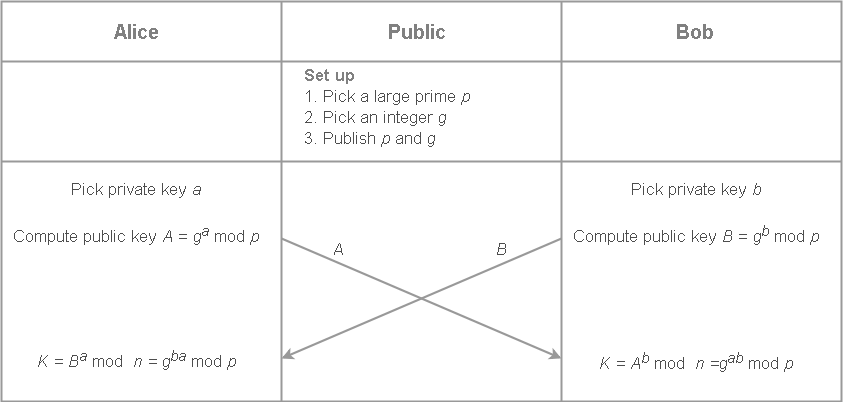
\includegraphics[width=14cm]{figures/dh.png}
	\caption{Simple Diffie-Hellman Key Exchange}
	\label{fig:dh}
\end{figure}

Alice and Bob will each pick a private key value and compute a public key value. The computed key value is sent over the insecure channel and Alice and Bob will both perform the same computation as previously \cite{crypto101}.


The Diffie-Hellman is vulnerable to man in the middle attack since there is no authentication taking place. There exist a solution to this problem using asymmetric key pairs and signing the messages being sent \cite{crypto101}.

\subsubsection{Key Derivation function}

Assume a secret key is established between two parties and is used to encrypt messages and exchange them over an insecure channel. An adversary listening might store all the messages being send even though he is not able to read them. However at some point he manages to compromise the secret key hence being able to decrypting every message ever sent.

To overcome the above scenario ephemeral keys are used. Such keys are short lived and are discarded after use.   

New secret keys can be generated using a \emph{Key Derivation Function} (KDF).
A KDF is a one way function that derives one or more randomized secret keys based on a secret key (or multuple) and optionally some input value \cite{crypto101}. Figure \ref{fig:kdf} illustrates this.

 \begin{figure}[H] 
 	\centering
 	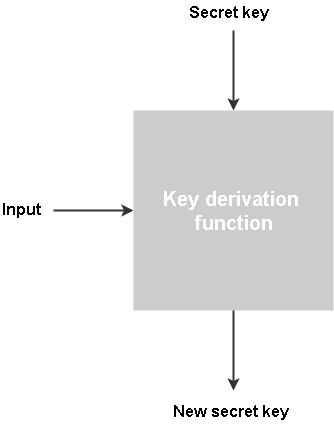
\includegraphics[width=8cm]{figures/kdf.png}
 	\caption{Key derivation function}
 	\label{fig:kdf}
 \end{figure}


A core concept in the Double Ratchet algorithm is KDF chains which build a chain of secret keys using KDF \cite{doubleratchet}. 


\subsubsection{Signal Protocol}

The Signal Protocol provides end-to-end encryption and was developed in 2013 and was first introduced in the app TextSecure\footnote{https://en.wikipedia.org/wiki/TextSecure}.

The Signal Protocol consists of two parts; The \emph{Triple Diffie-Hellman protocol} (TripleDH) and the Double Ratchet algorithm.

\paragraph{Triple Diffie-Hellman protocol}\label{tripledh}
Before the Double Ratchet algorithm can be used the two parties communicating need to agree on a shared secret key. In the Signal protocol this is achieved with Triple Diffie-Hellman protocol \emph{(TripleDH)}.

The Triple Diffie-Hellman protocol is a \emph{key agreement protocol}. It involves a server and two parties; Alice and Bob. 

The TripleDH protocol is characterized by three phases:

\begin{enumerate}
	\item \emph{Publishing keys:} A identity key and several prekeys belonging to Bob is published by him to a server.
	\item \emph{Sending initial message:} Alice sends an initial message to Bob. A prekey bundle is obtained by Alice from the server in order to send an initial message to Bob.
	\item \emph{Receiving initial message:} Alice's message is received and processed by Bob.
\end{enumerate}

\subparagraph{Publishing keys}
Bob needs to register a \emph{prekey bundle} to the server if he wants Alice to be able to send him messages. Alice will likewise have registered a prekey bundle so anyone can to anyone wants to start a message conversation with her.  
The prekey bundle exists of:

\begin{itemize}
	\item Identity key \emph{IK\textsubscript{B}}. This key is only published once by Bob.
	\item Signed prekey \emph{SPK\textsubscript{B}}. This key is reuploaded again after some period of time (eg. after each week or each month). 
	\item Prekey signature \emph{Sig(IK\textsubscript{B}, Encode(SPK\textsubscript{B}))}. This key is also reuploaded again like the signed prekey.
	\item Set of one-time prekeys \emph{(OPK\textsubscript{B}\textsuperscript{1}, OPK\textsubscript{B}\textsuperscript{2}, OPK\textsubscript{B}\textsuperscript{3}, ...)}. These keys are uploaded by Bob occasionally. Bob is informed by the server when there are few one-time prekeys left. 
	
	To ensure forward secrecy the private key of the one-time prekeys are deleted once Bob received messages that uses them. The signed prekey is deleted as well. However Bob might hold on to it for some time to get the messages that was delayed.  
\end{itemize}

\subparagraph{Sending initial message}
Alice retrieves Bobs public keys from the server. She receives one of Bob's single one-time prekey. The server deletes the one-time prekey that was send. It might be the case that all the one-time prekeys at the server has been used \cite{tripledh}.  


Alice verifies the prekey signature if the verification fails the protocol is aborted or else the following public keys are provided to generate a shared secret:

\begin{itemize}
	\item Identity key \emph{IK\textsubscript{A}}. Her own identity key. 
	\item Ephemeral key \emph{EK\textsubscript{A}}. The public key from a generated ephemeral key pair.
\end{itemize}


To generate the shared secret the following calculations are made:

\[DH_1 = DH(IK_A, SPK_B)\]
\[DH_2 = DH(EK_A, IK_B) \]
\[DH_3 = DH(EK_A, SPK_B)\]
\[DH_4 = DH(EK_A, OPK_B)\]
\[SK = KDF(DH_1 || DH_2 || DH_3 || DH_4)\]

There are performed atleast three Diffie-Hellman where \emph{DH\textsubscript{4}} is optional depending on if the server had more one-time prekeys.

Authentication is provided by \emph{DH\textsubscript{1}} and \emph{DH\textsubscript{2}} while \emph{DH\textsubscript{3}} and \emph{DH\textsubscript{4}} provides forward secrecy.

The figure \ref{tripledh} illustrates the calculations. 


\begin{figure}[H]
	\centering
	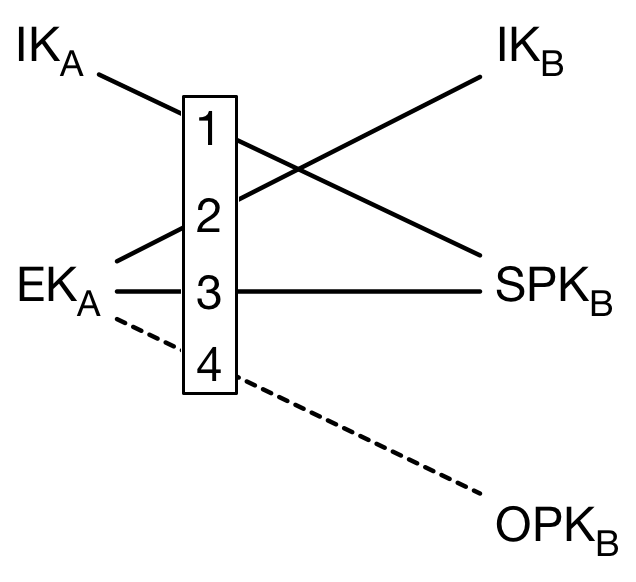
\includegraphics{figures/tripledh.png}
	\caption{Calculations of DH1-DH4 \cite{tripledh}.}
	\label{fig:tripledh}
\end{figure}

Alice then deletes the DH values and her private key associated to the ephemeral key to uphold forward secrecy and sends the initial message to Bob which consists of \cite{tripledh}: 

\begin{itemize}
	\item Cypher text with AEAD encryption  \footnote{https://en.wikipedia.org/wiki/Authenticated\_encryption} with \emph{associated data} using her own and Bob's identity keys.
	\item Her identity key \emph{IK\textsubscript{A}}.
	\item Her ephemeral key \emph{EK\textsubscript{A}}.
	\item Some identifiers to which of Bob's prekeys she used.
	
\end{itemize} 


\subparagraph{Receiving initial message}

When Bob receives Alice's initial message he performs the exact same calculations in phase two and derives the same shared secret key \emph{SK}.

Bob then decrypts the cypher text with the shared key and \emph{associated data} using his own and Alice's identity keys. If the decryption fails the protocol is aborted and \emph{SK} is deleted. Otherwise the protocol is complete and Bob deletes the one-time private prekey. 
The shared secret key can then be used for the Double Ratchet algorithm \cite{tripledh}.  

\paragraph{Double Ratchet algorithm}

After a shared secret key has been established the Double Ratchet algorithm can then be used to send and receive encrypted messages.

Each party has three chains; root chain, sender chain and receive chain. The chains are KDF chains and will take two keys as input (a KDF chain key and some other input key) and output new two keys (a new KDF chain key and some other output key). The KDF chain is illustrated in figure \ref{symkeyratchet}.

The algorithm has a \emph{Diffie-Hellman ratchet} step and \emph{symmetric ratchet} step and the chains are used across both steps.

\begin{itemize}
	\item \emph{Diffie-Hellman ratchet:} The parties exchanges new Diffie-Hellman public keys with the messages being sent. New secrets are then derived using Diffie-Hellman (DH). The secret that DH outputs is used as input to the root chain. The root chain then output new chain keys for the receiving and sending chains. 
	
	\item \emph{Symmetric ratchet:} The sending and receiving chains uses the chain keys derived from the root chain and for each message sent and received the chains are advanced. The output from the receiving and sending chains are keys for encrypting or decrypting messages. 
\end{itemize}


\subparagraph{Symmetric ratchet}
The symmetric ratchet provides message key through the receiving and sending chains. A message key is used for encryption or decryption of a message.

In the symmetric ratchet a single ratchet step is the calculation of the next key chain and message key. The inputs are the current chain key and a constant. Figure \ref{fig:symkeyratchet} illustrates two steps in a symmetric ratchet.

\emph{Forward secrecy} is provided since KDF is a one-way function and it is not possible to go backward and get the input chain key from the output chain key. However since the other input is simply a constant all future keys chain keys and message keys can be derived from an older chain key more specifically there is lack of backward secrecy.


\begin{figure}[H]
	\centering
	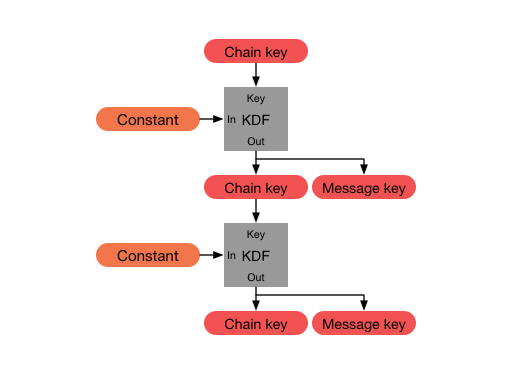
\includegraphics[width=10cm]{figures/symmetrickeyratchet.png}
	\caption{Symmetric key ratchet \cite{doubleratchet}.}
	\label{fig:symkeyratchet}
\end{figure}


\newpage
\subparagraph{Diffie-Hellman ratchet}

Double ratchet provides backward secrecy by comining the Symmetric ratchet with a Diffie-Hellman ratchet hence the name \emph{Double Ratchet}.

Every message from either party begins with a header which contains the sender's current ratchet public key. Whenever a new ratchet public key is received a new ratchet key pair is generated; a secret is derived through Diffie-Hellman with the input being the received ratchet public key and the ratchet private key from the new generated key pair.

Alice starts a conversation with Bob and uses his published public key as a ratchet public key. Alice then generates a new ratchet key pair and derives a shared secret key using Diffie-Hellman and would that as input to her \emph{sending chain}. Alice then sends her new ratchet public key to Bob. At the receiving end Bob derives the same shared secret which would be the input to his \emph{receiving chain}. Alice's sending chain and Bob's receiving chain share the same secret hence he can derive the message key and decrypt the message sent from Alice. When Bob sends a reply to Alice he would generate a new ratchet key pair and derive a new secret which would be input to his \emph{sending chain}.

Figure \ref{fig:dhratchet1} shows an ongoing message exchange with new secrets being derived and the sending and receiving chains being advanced.

\begin{figure}[H]
	\centering
	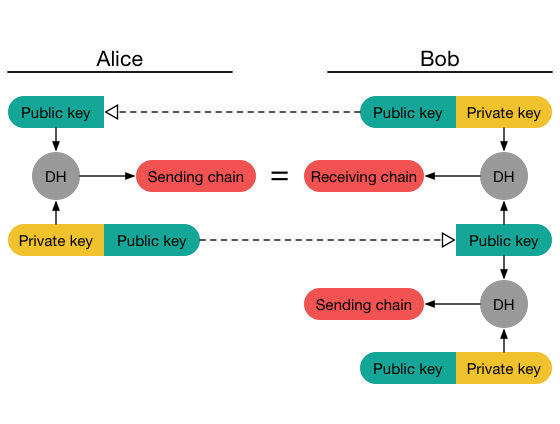
\includegraphics[width=9cm]{figures/dhratchet5.png}
	\caption{Diffie-Hellman ratchet \cite{doubleratchet}.}
	\label{fig:dhratchet1}
\end{figure}


When Alice receive the reply from Bob she would perform the exact same steps. This ultimately results in a continous loop of generating new ratchet key pairs and using Diffie-Hellman to derive the same shared secret key. A continuation is shown in figure \ref{fig:dhratchet2}

\begin{figure}[H]
	\centering
	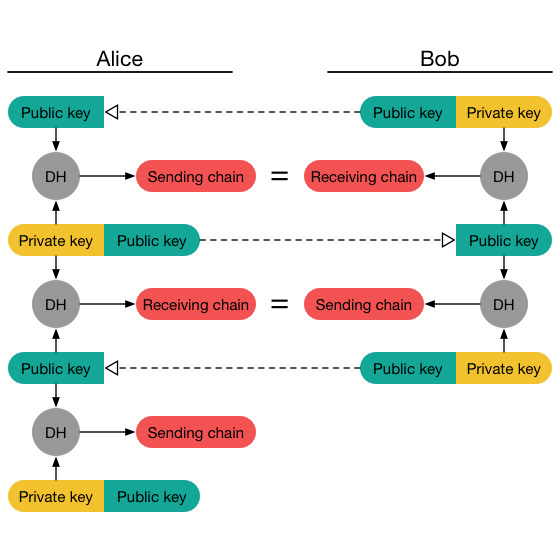
\includegraphics[width=9cm]{figures/dhratchet6.png}
	\caption{Continuation of Diffie-Hellman ratchet  \cite{doubleratchet}.}
	\label{fig:dhratchet2}
\end{figure}


As mentioned in the beginning of the Double Ratchet section the Diffie-Hellman ratchet does have a root chain which would provide inputs to the sending and receiving chains. A more correct view of the process in Diffie-Hellman is shown in figure \ref{fig:dhratchetcon}. 


\begin{figure}[H]
	\centering
	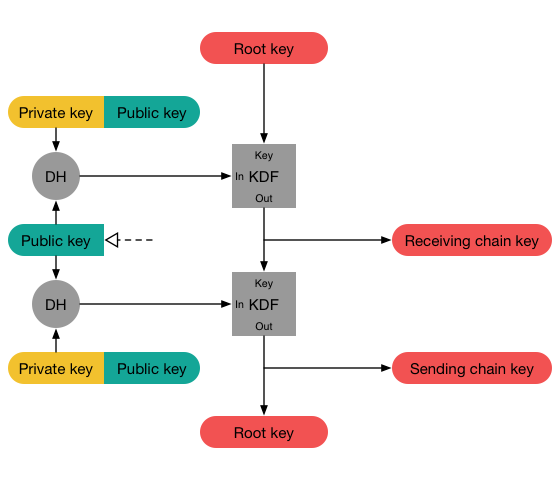
\includegraphics[width=9cm]{figures/dhratchet7.png}
	\caption{Diffie-Hellman ratchet 7 \cite{doubleratchet}.}
	\label{fig:dhratchetcon}
\end{figure}

\paragraph{Double ratchet}

When combining Diffie-Hellman ratchet and symmetric-key ratchet the result is the Double ratchet.

\begin{itemize}
	\item When sending or receiving a message the corresponding message key is derived by performing a symmetric-key ratchet step.
	\item Upon receiving a new ratchet public key the Diffie-Hellman ratchet step performed right before the symmetric-key ratchet step with the goal of replacing old chain keys with new ones.  
\end{itemize}

Assume that the message exchanged is a continuation from the TripleDH key exchange described in section \ref{tripledh}. Alice had sent an initial message. The initial ratchet public key would be Bob's signed prekey \emph{SPK\textsubscript{B}} and the new ratchet key pair would be the Alice's ephemeral key pair that she generated. Alice calculated a shared secret which is the \emph{root key}. She then generates a new ratchet key pair and takes the output from Diffie-Hellman and use it as input for the \emph{root chain}. The root chain then outputs a new root key \emph{RK} and a sending chain key {CK}.

The figure \ref{doubleratchet1} depicts this with a view of Alice's chains.


\begin{figure}[H]
	\centering
	
\includegraphics[width=10cm]{figures/doubleratchet1.png}
	\caption{Double ratchet 1 \cite{doubleratchet}.}
	\label{fig:doubleratchet1}
\end{figure}

When Alice then sends a message \emph{A1} the symmetric-key ratchet step will return a new chain key and a message key. The message can then be encrypted with the message key.

\begin{figure}[H]
	\centering
	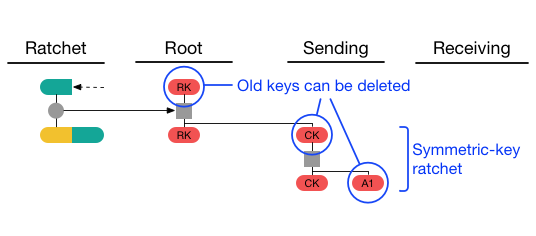
\includegraphics[width=10cm]{figures/doubleratchet2.png}
	\caption{Double ratchet 2 \cite{doubleratchet}.}
	\label{fig:doubleratchet2}
\end{figure}

Next Alice receives a message \emph{B1} from Bob. The message header contains a new ratchet public key and a Diffie-Hellman ratchet step is performed. New sending and receiving chain keys are derived and followed by a symmetric-key ratchet step to derive the receiving message key to decrypt the message.

\begin{figure}[H]
	\centering
	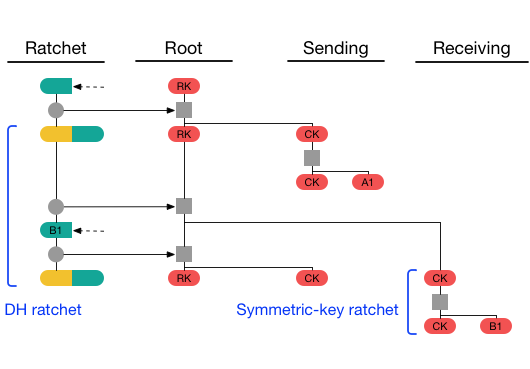
\includegraphics[width=10cm]{figures/doubleratchet3.png}
	\caption{Double ratchet 3 \cite{doubleratchet}.}
	\label{fig:doubleratchet3}
\end{figure}





\newpage
\section{Matrix}

\subsection{Goals}

\subsubsection{Short term goal}

\subsubsection{Long term goal}
% https://www.youtube.com/watch?v=-ofZMnKkp_Y 5:00 , 18:30

\subsection{How does it work?}

\subsection{Architecture}

\subsection{Matrix specification}

\subsection{End-to-end Encryption}





\newpage
\section{Information Flow Control} %mere konkret og teknisk
%Selvom jeg ikke kiggr på fx trafic analysis så er det vigtigt at nævne og påpege det ikkeer noget jeg løser

\subsection{The Lattice Model}
adsadsad

\subsection{Noninterference}
dasdsa

\subsection{Static policies}


sadsad
\subsection{Dynamic policies}
sadsadsad


\subsection{Declassification}
Taking some specific information and changing it to a lower security classification.

Identify: What to classify, who declassifies, where the declassification happens and when the declassification happens

\section{Summary}


\chapter{Analysis}\label{analysis}
This chapter consists of two parts. The first part will provide an evaluation of the Matrix security model and relies on the paper \emph{SoK: Secure Messaging} \cite{sok} and \emph{The Olm Cryptographic Review} by NCC Group \cite{ncc}. 

The second part provides a preliminary analysis of the IFC tools, the selection of Paragon and the rationale behind it, and a further analysis of the selected tool Paragon.


\section{Evaluation of Matrix security model}
The security of matrix will be evaluated in the context of secure messaging. An evaluation framework has been proposed in the paper \emph{SoK: Secure messaging} which the evaluation will be loosely based on. 

The evaluation framework covers several areas with \emph{conversation security} being the most relevant for this evaluation. The area \emph{conversation security} describes three categories; \emph{Security and Privacy}, \emph{Adoption}, and \emph{Group Chat}. Obviously the most relevant category for the evaluation is \emph{Security and Privacy}
\\
\\
Matrix provides end-to-end encryption by using the Olm and Megolm library with the former being an implementation of the Double Ratchet algorithm also known as the Signal Protocol, and the latter being the algorithm used for group chat. 

Olm is used for securely exchanging message keys/session keys during group chat and is vital part of the end-to-end encryption in Matrix.

Before the Matrix protocol is evaluated the Signal Protocol will be considered. 

%\subsection{Threat model} Describe the threat model in SoK

\subsection{Signal Protocol}
Olm is an implementation of the Signal Protocol. The Signal Protocol is a messaging protocol with end-to-end encryption between two devices. 

Section xx provides a list of security properties relevant for \emph{conversation security}. These security properties is used for evaluating a secure messaging protocol such as the Signal Protocol.
%Any messaging application that provides end-to-end encryption is likely an implementation of  the protocol 

The table below shows an evaluation of the Signal Protocol (previously known as TextSecure) \cite{sok}. 

\begin{figure}[H]
	\hspace*{-1.7cm} 
	\centering
	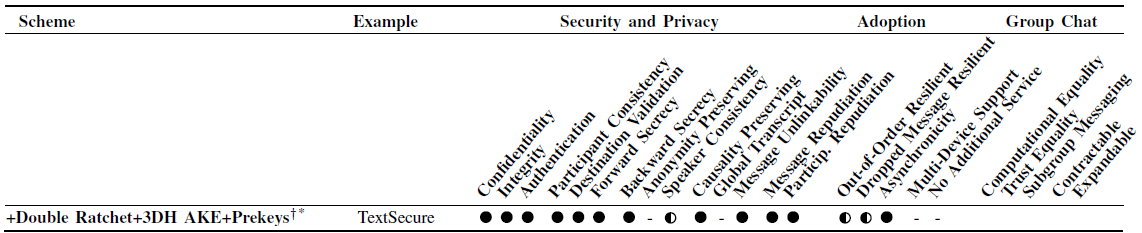
\includegraphics[width=16cm]{figures/framework_signal.png}
	\caption{Evaluation of Signal (TextSecure) \cite{sok}.}
	\label{fig:framework_signal}
\end{figure}


%Explain how they provide the properties or why they don't


\subparagraph{Confidentiality} When a message is sent using the Signal Protocol then only the intended recipient can read the message. The senders sending ratchet and receivers receiving ratchet will derive the same message key hence only the two parties will be able to encrypt the messages. 

\subparagraph{Integrity} The receiver will only accept a message if it is successfully decrypted hence if in transit a message was modified then the message would be rejected.

\subparagraph{Authentication} The decryption of a message also gives authentication guarantees since only the intended recipient could compute the message key.

\subparagraph{Forward secrecy} The symmetric ratchet ensures forward secrecy. If a chain session key is compromised then the previous keys can not be generated since the ratchet is one way cryptographic hash function hence secrecy is provided for all previous send messages.  

\subparagraph{Backward secrecy} Diffie-Hellman ratchet have the self-healing property and will generate a new chain session key for the symmetric ratchet hence if a chain key is compromised then secrecy for future messages is still provided because a new chain ratchet key will be generated.

\subparagraph{Anonymity preserving}

Anonymity preservation is lost in the Signal Protocol since the initial key agreement requires long-term public keys hence making them observable during Triple-DH. However \textbf{\emph{participant consistency}} is provided by Triple-DH \cite{sok}. %How?
%Without participant consistency, identity misbinding attacks might be possible. Unknown key share attack

\subparagraph{Speaker consistency}
This property is partially provided through the key evolution of the ratchets. If a message is dropped then it is not possible to generate message keys for future messages. This also makes the protocol partially have the property \emph{\textbf{Dropped message resilence}}. It will also not go unnoticed if a message is received out of order since this will result in the message's key being an unexpected key. Hence the recipient have to store expired keys to decrypt delayed messages. This makes the property \emph{\textbf{Out-of-order resilient}} only partially provided \cite{sok}.

\subparagraph{Global transcript} 
In an asynchrounous messaging protocol there is no global transcript. Both participants have to be online to receive messages hence the participants will not have all the messages if one of them is offline. This is a result of having the \textbf{\emph{Asynchronicity}} property.

\subparagraph{Deniability properties}

Since the ratchet session keys are used for encrypting messages and not the long-term public keys the properties \textbf{\emph{Message unlinkability}} and \textbf{\emph{Message repudiation}} are provided. 


\subparagraph{Other properties}

\begin{itemize}
	\item \textbf{\emph{Participant repudiation}}. Triple-DH achieves full participant repudiation since anyone can forge a transcript between any two participants \cite{sok}.
	\item \textbf{\emph{Destination validation}}. The Deffie-Hellman ratchet provides this property since the recipients public key is used to generate the chain key \cite{sok}. % Is this true?
\end{itemize}


The evaluation shows that several security properties are provided with the important ones being confidentiality, integrity, authentication, forward secrecy, backward secrecy. 

Furthermore a formal analysis have been made on the Signal Protocol that proves the protocol is free from any major flaws and it satisfy the following security properties; confidentiality, authentication and secrecy \cite{Signal}. 

%The next section provides a brief summary of the analysis.

%\newpage
%
%\subsubsection{Summary of the security analysis of Signal Protocol}
%\emph{**NOTE: Is this section even relevant to have in the report? **}
%
%
%As described earlier in section xx the Signal Protocol consists of three stages.
%
%\begin{itemize}
%	\item Initial stage (Triple-DH). For establishing a shared secret. 
%	\item Deffie-Hellman ratchet. For generating session key. 
%	\item Symmetric ratchet. For generating message key.
%\end{itemize}
%
%
%
%\paragraph{Threat model}
%The threat model defined in the analysis assumes that the adversary have full control over the network.
%
%The adversary can observe traffic over the network and can drop and send messages.
%
%For an adversary to break security he must be able to
%
%For an adversary to break security he must obtain 
%
%In assymmetric messaging a party can be offline over 
%
%\paragraph{Security properties}
%
%The high-level properties we aim to prove are secrecy and authentication of message keys
%
%\begin{itemize}
%	
%	\item Secrecy. If Alice and Bob complete an exchange to generate a key k, nobody other than Alice and Bob should be able to learn anything about k. Forward secrecy are not explicit goals; instead, derived session keys should remain secret under a variety of compromise scenarios.
%	\item (Implicit) Authentication. If Alice believes that she shares the key k with Bob, nobody other than Bob should be able to learn anything about k. Note that this property is implied by secrecy. Authentication will be implicit meaning that only the intended party could compute the key rather than explicit (get a guarantee that the intended party did compute the key).
%\end{itemize}
%
%%and thereby distinguish any fresh message encryption key from random
%
%
%As described earlier a group chat is represented by a session which has three stages; initial exchange, asymmetric and symmetric. Each stage will generate a key 
%
%
%By proving that the session keys generated at each stage are key indistinguishable it can be argued that the session keys at each stage are safe...
%
%
%We find if the above goals are fulfilled by looking at the freshness of the session keys in the different stages. By defining under what conditions the session keys are fresh and by proving that they indeed are fresh then it has been proved that the above security properties are provided. 
%
%
%\paragraph{Freshness and cleanness} 
%
%Our goal when defining fresh is to describe the best security condition that might be provable for each of
%Signal’s message keys based on the protocol’s design; here, “best” is with respect to the maximal combinations
%of secrets learned by the adversary.
%That is, we use the structure of the protocol to infer which attacks cannot
%possibly be prevented, and rule them out by restricting the adversary.
%
%For each session there are different definition of freshness.
%
%The cleanness predicate defines under what conditions the session keys are .....
%
%
%
%\subparagraph{Stage 0}
%We can prove the security of the stage 0 key (output by the triple key exchange during session setup) if one of the following is upheld cleanLM(u,i), cleanEL(u,i,0), cleanEM(u,i,0).
%
%\subparagraph{Asymmetric stages}
%In this stage there are two types; asym-ir (sending) or asym-ri (receiving).
%
%By satisfying the cleanness predicates for each type of state we can prove the security of this stage.
%
%Most cases are of the form cleanEE, and for these we obtain a probability bound by replacing the DH ratchet keys and shared secrets with values from a GDH challenger.
%
%The only case not of this form involves clean\_state, which describes a scenario where both recent ratchet keys were compromised but the previous stage was still secure. Secrecy here is intuitive, and the bound follows from an inductive argument: if an adversary could win in this manner, then, assuming GDH and ROM security, there is an adversary which could win against the previous stage.
%
%
%\subparagraph{Symmetric stages}
%To ensure security of session key in this stage we only need to consider the following case. We replace the keys used to initialise the current sending chain with uniformly random values, since an adversary who could detect this could win against that
%previous stage.
%\\
%\\
%The proof for the above is provided in detail in the paper \emph{A Formal Security Analysis of the Signal Messaging Protocol} \cite{Signal}.


\subsubsection{Application variants}

The Olm library used by Matrix is a variant of the Double Ratchet algorithm. The custom variants invites important changes in need to be analyzed independently. WhatsApp variant of the protocol has a retransmission mechanism which is vulnerable. 
% if Bob appears to change his identity key, clients will resend messages encrypted under the new value.Hence, an adversary with control over identity registration can disconnect Bob and replace his key, and Alice will re-send the message to the adversary.  
The further evaluation relies upon the the security assessment on Matrix. 

\subsection{Matrix protocol}




\subsubsection{Group chat}
The Double Ratchet algorithm is meant for one-to-one chatting and is not practical for group chatting. %why not?

For direct conversation Matrix uses Olm library which is an implementation of the Double Ratchet algorithm. For group chats the Megolm library is used. 

It is more difficult to evaluate the Matrix protocol because they as well do not specify any detailed security goal and there is at this point of writing no formaæ analysis of their implementation of the Double Ratchet algorithm.


List problems with group chat 

\begin{itemize}
	\item Lack of post compromise security
\end{itemize}

There is an tradeoff on security and usability and the security is decreased for group chats. %8.30

As of this moment of writing there exist no implemented protocol that solves these issues in group chat. However recent research has proposed solutions with early implementations for these problems with IETF leading the research on the standard on \emph{Messaging Layer Security}. Matrix has expressed awareness of the protocol and a possibility of adaption in the future.

\subsubsection{Olm}
Olm is an implementation of the Double Ratchet algorithm and plays a major role in the Megolm library which is used by Matrix group messaging. 

The security assessment provides a review of the Olm and Megolm libraries. However there exist no work that verifies if Olm correctly implements the Double Ratchet described earlier.

Vulnerabilities found in the security assessment. 

\paragraph{Unknown Key Share attack}

In this variant of the unknown key-share (OKs) attack, an attacker will allow highly targeted, known messages to be sent to Bob. In this scenario, Bob will still believe he is talking with Alice. Here, two parties (Donald and Mallory), who may be the same person, will collude against Alice in a group chat situation (Megolm). Donald will be performing the unknown key-share attack. Mallory will be an instigator (attempting to elicit messages from Alice that will later be sent to Bob) who will be able to read the contents of the group chat.

\subsubsection{Megolm}
% The way Megolm works is to give every sender in the room its own encrypted ratchet (‘outbound session’), so every device encrypts each message once based on the current key given by their ratchet (and then advances the ratchet to generate a new key).  Meanwhile, the device shares the state of their ‘outbound session’ to every other device in the room via the normal Olm ratchet in a 1:1 exchange between the devices.  The other devices maintain an ‘inbound session’ for each of the devices they know about, and so can decrypt their messages.  Meanwhile, when new devices join a room, senders can share their sessions according to taste to the new device – either giving access to old history or not depending on the configuration of the room.



Conceptually, when you first send a message in an encrypted room, your Riot client generates a random key to encrypt your message, sends the encrypted message to the server, and then sends the decryption key to all the devices in the room that should be allowed to decrypt the message. Of course, the decryption key is sent encrypted (based on the device's unique key, which you verified above) so that it cannot be intercepted. The recipient then fetches the message decryption key and the encrypted message and decrypts the message.

In order to avoid having to re-send decryption keys to every device for every message you send, Matrix's encryption system includes a method for generating a new key based on an old key. So for the next message you send, your Riot client will use that method on your previous encryption key to generate a new key, and the recipients will use the same method and generate the same key, so that when you send a message encrypted using the new key, the recipients can decrypt the message without any extra key exchange. The new key will only need to be sent to any new devices that showed up in between when the first message was sent and when the second message was sent.

Riot will occasionally start from scratch, generating a new random key and sending it to all the devices in the room. This happens, for example, whenever someone leaves a room, after you have sent a certain number of messages, or after a certain amount of time.

\paragraph{Message Replays}
A message can be decrypted successfully multiple times. This means that an attacker can re-send a copy of an old message, and the recipient will treat it as a new message.

To mitigate this it is recommended that applications track the ratchet indices they have received and that they reject messages with a ratchet index that they have already decrypted.

\paragraph{Lack of Transcript Consistency}
In a group conversation, there is no guarantee that all recipients have received the same messages. For example, if Alice is in a conversation with Bob and Charlie, she could send different messages to Bob and Charlie, or could send some messages to Bob but not Charlie, or vice versa.

Solving this is, in general, a hard problem, particularly in a protocol which does not guarantee in-order message delivery. For now it remains the subject of future research.

\paragraph{Lack of Backward Secrecy}
Once the key to a Megolm session is compromised, the attacker can decrypt any future messages sent via that session.

In order to mitigate this, the application should ensure that Megolm sessions are not used indefinitely. Instead it should periodically start a new session, with new keys shared over a secure channel.

\paragraph{Partial Forward Secrecy}
Each recipient maintains a record of the ratchet value which allows them to decrypt any messages sent in the session after the corresponding point in the conversation. If this value is compromised, an attacker can similarly decrypt those past messages.

To mitigate this issue, the application should offer the user the option to discard historical conversations, by winding forward any stored ratchet values, or discarding sessions altogether.

\paragraph{Dependency on secure channel for key exchange}
The design of the Megolm ratchet relies on the availability of a secure peer-to-peer channel for the exchange of session keys. Any vulnerabilities in the underlying channel are likely to be amplified when applied to Megolm session setup.

For example, if the peer-to-peer channel is vulnerable to an unknown key-share attack, the entire Megolm session become similarly vulnerable. For example: Alice starts a group chat with Eve, and shares the session keys with Eve. Eve uses the unknown key-share attack to forward the session keys to Bob, who believes Alice is starting the session with him. Eve then forwards messages from the Megolm session to Bob, who again believes they are coming from Alice. Provided the peer-to-peer channel is not vulnerable to this attack, Bob will realise that the key-sharing message was forwarded by Eve, and can treat the Megolm session as a forgery.

A second example: if the peer-to-peer channel is vulnerable to a replay attack, this can be extended to entire Megolm sessions.

% Lack of backward secrecy is problematic for the prototype.

%Enforcing new session start every time a patient journal is sent. Could it be enforced with IFC?




\subsubsection{Evaluation}
The evaluation framework in the paper \emph{SoK: Secure Messaging} defines \emph{Conversation Security} as a problem area which contains the following main groups; \emph{Security and Privacy Featues}, \emph{Adoption}, and \emph{Group Chat}.


\begin{figure}[H]
	\centering
	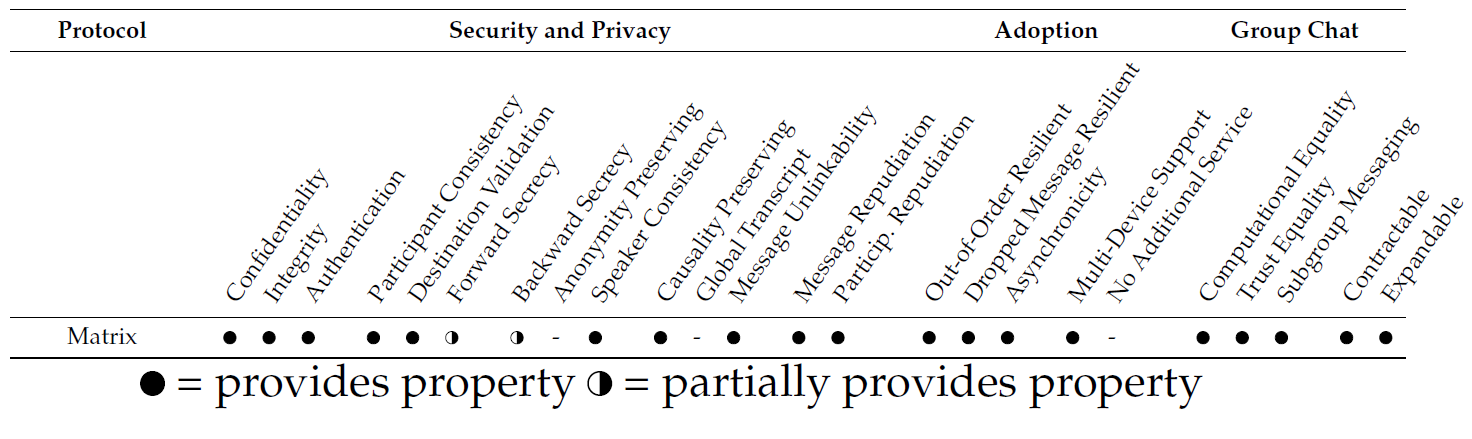
\includegraphics[width=12cm]{figures/framework.png}
	\caption{Evaluation of Matrix Security.}
	\label{fig:framework}
\end{figure}

\subparagraph{Confidentiality} When a message is sent using the Signal Protocol then only the intended recipient can read the message. The senders sending ratchet and receivers receiving ratchet will derive the same message key hence only the two parties will be able to encrypt the messages. 

\subparagraph{Integrity} The receiver will only accept a message if it is successfully decrypted hence if in transit a message was modified then the message would be rejected.

\subparagraph{Authentication} The decryption of a message also gives authentication guarantees since only the intended recipient could compute the message key.

\subparagraph{Forward secrecy} The symmetric ratchet ensures forward secrecy. If a chain session key is compromised then the previous keys can not be generated since the ratchet is one way cryptographic hash function hence secrecy is provided for all previous send messages.  

\subparagraph{Backward secrecy} Diffie-Hellman ratchet have the self-healing property and will generate a new chain session key for the symmetric ratchet hence if a chain key is compromised then secrecy for future messages is still provided because a new chain ratchet key will be generated.

\subparagraph{Anonymity preserving}

Anonymity preservation is lost in the Signal Protocol since the initial key agreement requires long-term public keys hence making them observable during Triple-DH. However \textbf{\emph{participant consistency}} is provided by Triple-DH \cite{sok}. %How?
%Without participant consistency, identity misbinding attacks might be possible. Unknown key share attack

\subparagraph{Speaker consistency}
This property is partially provided through the key evolution of the ratchets. If a message is dropped then it is not possible to generate message keys for future messages. This also makes the protocol partially have the property \emph{\textbf{Dropped message resilence}}. It will also not go unnoticed if a message is received out of order since this will result in the message's key being an unexpected key. Hence the recipient have to store expired keys to decrypt delayed messages. This makes the property \emph{\textbf{Out-of-order resilient}} only partially provided \cite{sok}.

\subparagraph{Global transcript} 
In an asynchrounous messaging protocol there is no global transcript. Both participants have to be online to receive messages hence the participants will not have all the messages if one of them is offline. This is a result of having the \textbf{\emph{Asynchronicity}} property.

\subparagraph{Deniability properties}

Since the ratchet session keys are used for encrypting messages and not the long-term public keys the properties \textbf{\emph{Message unlinkability}} and \textbf{\emph{Message repudiation}} are provided. 


\subparagraph{Other properties}

\begin{itemize}
	\item \textbf{\emph{Participant repudiation}}. Triple-DH achieves full participant repudiation since anyone can forge a transcript between any two participants \cite{sok}.
	\item \textbf{\emph{Destination validation}}. The Deffie-Hellman ratchet provides this property since the recipients public key is used to generate the chain key \cite{sok}. % Is this true?
\end{itemize}


\subsection{End-to-end security}
It can be argued that some of the Matrix shortcomings can be configured on the application layer. This puts a lot of responsibility on the application and that it is configured correctly. 

Even if the application using Matrix is configured correctly and give the best guarantee of forward and backward secrecy this not the end of security. 

Dynamic policies?


\begin{figure}[H]
	\centering
	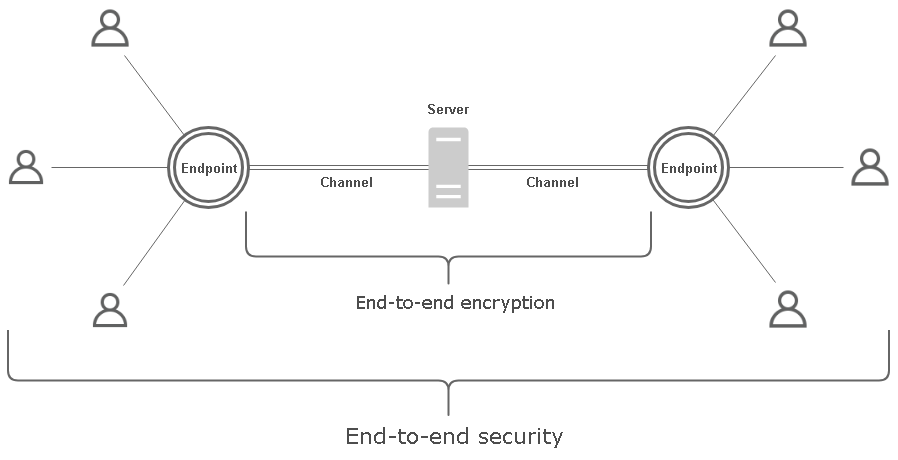
\includegraphics[width=12cm]{figures/e2esecurity.png}
	\caption{End-to-end security.}
	\label{fig:e2esecurity}
\end{figure}


Recently two technical directors from the Government Communication Headquarters of United Kingdom released an essay arguing that the software vendors could grant access to group chat by inserting the government as a hidden silent participant in a chat hence not weakening the encryption \cite{gchq}.


Explain how some of the shortcomings in Matrix can be solved with IFC.The initial state ratchet is never ratcheted?

\subsection{Summary}






% Tools issue: java sdk for matrix is beta and not fully implemented. 
% Best supported sdk is for javascript or python. Problem of running javascript code or python code with Paragon (java)
% Maybe better to use JSFlow instead 


%\section{Survey of IFC Tools}
%Having established that end-to-end security is not the end of security we will now look at Information-Flow Control tools. 

%The approach to the section will be from a programmers perspective hence usability and practicality will play a role in which IFC tool is chosen. 

%\subsection{JIF}

%\subsection{Paragon}

%\subsection{JSFlow}
%Not possible to use Matrix library with JSFlow because of missing support for libaries such as require (in node). Also overhead with configuring JSFlow to be the interpretor.

%Swift, SIF, FlowR, JFlow, LIO


%\subsection{Selection of IFC tool}
%The selection of the IFC tool used for developing the prototype is based the following defined parameters.
%The selection of IFC tool put emphasis on the practical usage in combination with Matrix. 

%\subsection{Paragon analysis}

%\subsection{Summary}


%\section{Summary}
%In this chapter the Matrix security model has been evaluated. Matrix provides end-to-end security and uses the Double Ratchet algorithm by Signal. The evaluation found that there are no major flaws in the design. To achieve end-to-end security the endpoints need to be secured as well \cite{Sabelfeld2003} this leads us to the chapter's second part. The chapter analyzed information-flow control tools and justifies the selection of Paragon which the prototype is programmed in. 

%\chapter{Implementation}\label{design}
%
% This chapter presents the implementation of a distributed system running on Matrix and developed with Paragon as described in the criterias.

This chapter describes the implementation of the prototype. The prototype is a system for sending and retrieving patient journals among different hospitals. The system relies on Matrix as the secure communication channel and storage.


\section{Journal system}

% Describe the requirements for the journal system.
The journal system is inspired by the Danish E-journal system as described in section \ref{intro}. A journal system serves an important purpose by providing patient journals to different hospitals and clinics. If a patient arrives at the ER and the doctor cannot access the patient's journal then the treatment of the patient gets problematic. A doctor might miss out on important details about the patient or even worse prescribe medication that might give the patient an allergic reaction. The availability of a patient journal is a necessity however the number of medical employees that have access to such a journal has raised privacy concerns. Around 90.000 medical employees have access to patient journals. Consider the scenario where a patient gets referred to a physiotherapist with muscle pain. When the therapist opens the journal the full medical history will be present; if the patient had received psychiatric treatment those session would be readable too. Furthermore a patient journal is accessible by a large number of unrelated medical employees with the only prevention mechanism being logging and audit trails.


The lack of secure information flow is evident and the prototype demonstrates how Information-Flow control can be leveraged to enforce security policies concerning the information. The journal system is a small distributed system where Hospitals can send, receive and store patient journals. Matrix provides the distributed structure and is responsible for securely storing and transmitting the journals. Paragon provides secure information flow at the endpoints hence providing end-to-end security. 
The following requirements are defined for the prototype:

\begin{itemize}
	\item A patient journal contains low (public), medium (confidential) and high (secret)  information.
	\item A patient journal is send and received securely over a channel.
	%\item A patient journal can only be appended to. 
	\item Hospitals have shared access to patient journals. 
	\item A hospital has two actors: Doctor and Secretary.
	\item A secretary can only see low parts of the journal.
	\item A secretary can edit the public parts of a journal.
	\item A doctor can see the everything up to confidential information.
	\item A doctor must have the patient in care to gain the journal's secret information.
	\item A doctor can edit the public part and confidential parts of a patient journal.
	\item A doctor can only add to a secret fields in a patient journal if the patient has been referred to the doctor.
\end{itemize}

The following non-functional requirements are defined:

\begin{itemize}
	\item Confidentiality: the system must ensure the confidentiality throughout the system according to the security policies at all times.
	\item Integrity: the system must ensure that only intended actors can modify the specific parts of a patient journal.
\end{itemize}

The current journal systems allows medical employees to access the journals from anywhere. The prototype makes the assumption that the system can only be used within hospitals. Furthermore access for patients to their journal is not supported.

\subsection{System design} \label{systemdesign}

The system is distributed and allows to run multiple clients to send and retrieve patient journals. The system consists of two components; \emph{Matrix} and the \emph{client}. The Matrix component encapsulates the Matrix SDK and provides an interface to Paragon. The client component consumes that interface and can be considered as the endpoint in a communication channel. The client component provides secure information flow for data received through Matrix. Without the interface it would not be possible to achieve end-to-end security in the system. 
The component diagram in figure \ref{fig:matrix_component} depicts this.

\begin{figure}[H] 
	\hspace*{-1cm}
	\centering
	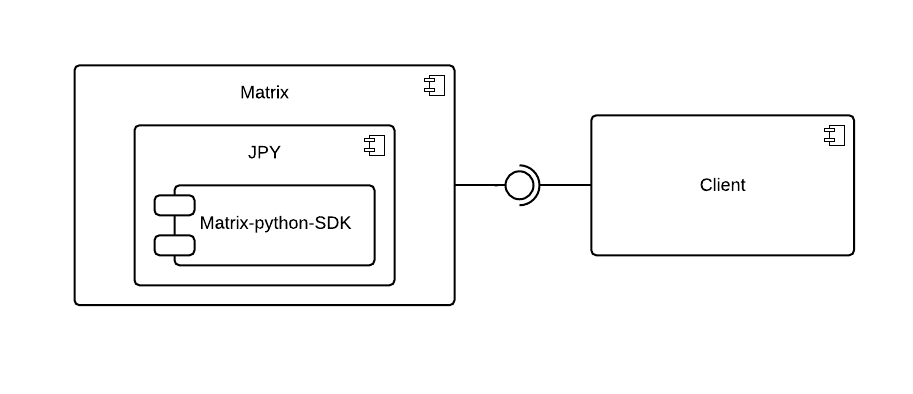
\includegraphics[width=14cm]{figures/matrix_component.png}
	\caption{Component diagram for the system}
	\label{fig:matrix_component}
\end{figure}

Matrix provides several SDK libraries that client application can be build on top of. The most prominent is the Javascript Matrix SDK. It is the best maintained with the largest feature set however it is not compatible with the Java based Information-Flow Control tool Paragon. A Java Matrix SDK exists but it is an early alpha version with end-to-end encryption not implemented yet. The Python Matrix SDK is another major SDK with support for end-to-end encryption in beta. The Python Matrix SDK is used in the Matrix component through a Java-Python bridge \emph{JPY} that can embed Python code in Java as shown in the Matrix component in figure \ref{fig:matrix_component} 




\subsubsection{Matrix}
%Matrix API's
% A lot of things are handled under the hood by the matrix SDK.
Matrix is an important component in the system. It manages the transmission and storage of patient journals through rooms while managing end-to-end encryption. The encryption mechanism is automatically provided and the SDK manages the session keys under the hood.  As described in section \ref{matrix:architecture} a room is a conceptual place for sending an receiving events and events can be any of any structure. The event history in a rooms is replicated at each homeserver. 

The following design choices and assumptions are made regarding Matrix and the system: 

\begin{itemize}
	\item A homeserver represents a hospital server that replicates the history of a patient journal. 
	\item A room represents a single patient journal's version history.
	\item An event represents a patient journal.  
	\item The latest event in a room is the global state of the patient journal.
	\item A hospital is represented by a single matrix user that participates in a room.
	\item A hospital's matrix user is used by doctors and secretaries to access patient journals. 
\end{itemize}


The room can be considerably large since many different types of hospitals needs access to a patient journal. This puts a lot of responsibility on securing the endpoints but also adds concern to who controls the rooms and how hospitals are added. It is assumed that a central authority would be managing all room whom all participants in the room trust. That authority would be the government which are responsible for creating and managing the rooms. Only the authority can invite and remove Hospitals from a room. Hospitals can only join a room if they have been invited.


\subsubsection{Client}

A client represents a hospital with a set of employees that can view some journals. The hospital subscribes to rooms in Matrix that the employees can fetch. The client is a simple console application and is preconfigured to run as a hospital. During program start a list of employees is presented. It is assumed that by selecting an employee the user login as that employee. The user is then presented a list of patients that can be selected. The list is provided by the hospital that keeps track of all journals in a \emph{map} with \emph{SSN} (Social security number) as the key and \emph{matrix room ID} as the value. When the user selects a journal; it is first retrieved from Matrix and the user then receives the journal. It is determined what tasks the user can perform and depending on the user's role the journal can be partially or fully accessible 

Figure \ref{fig:journalsystem} depicts the class diagram for the system.


\begin{figure}[H] 
	\hspace*{-1.3cm}
	\centering
	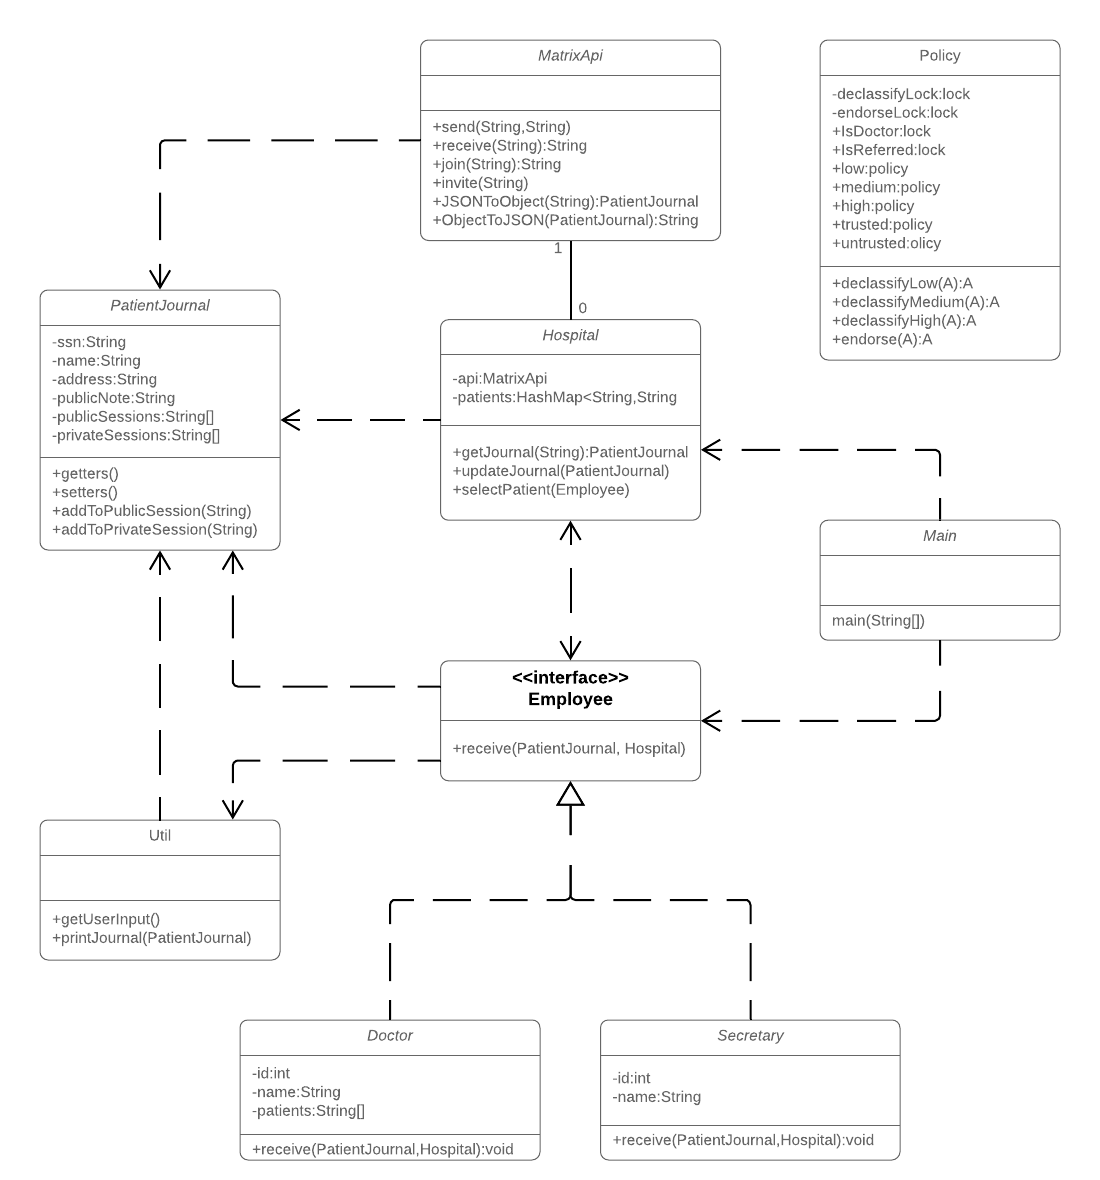
\includegraphics[width=14cm]{figures/journalsystem_class.png}
	\caption{Class diagram for the Journal system}
	\label{fig:journalsystem}
\end{figure}





\subsubsection{Limitations} \label{concurrentwrites}

%Incompatibility with Paragon


A design problem is the concurrent writes to a journal from multiple hospital. Before writing to a journal; the latest version of the journal in Matrix is first retrieved and then the writes are appended to the journal. However multiple hospitals might have retrieved the latest journal and different doctors might have committed changes to the journal and send it to Matrix hence one of the writes would be lost since only the latest journal is retrieved. A solution to this would be extending the rooms with version control functionality that would track and combine the changes made to a journal.


% It is assumed that a version control mechanism is in place and the latest journal received is always up to date.
% Solution merging data like version control systems like git.

\section{Paragon implementation}

\subsection{Matrix API}

The Matrix API implementation was briefly described in section \ref{systemdesign}. The API is implemented in Java using the foreign language binder JPY to leverage the Matrix Python SDK and makes it possible to use it with Java/Paragon. Without the API it would not be possible to use Matrix with Paragon. To be able to use the API; a Paragon \emph{signature} must be provided. In fact a signature file has to be specified to use any external Java class. The \emph{MatrixApi} signature file is specified as such:

\begin{lstlisting}
public native class MatrixApi<policy p> {
	!p void send(?p String message, ?p String room);
	?p String retrieve(?p String room);
	?p String objectToJSON(?p PatientJournalD object);
	?p PatientJournalD JSONToObject(?p String json);
}
\end{lstlisting}

The signature file describes that the \emph{MatrixApi} class takes a type argument \emph{policy} which specifies what policy the API should enforce. Note that Paragon cannot assert if the external class will respect the policies.

The annotation \emph{?} and \emph{!} represents \emph{read} and \emph{write} effects, and will be explained in the next sections.
 
\subsection{Policies}\label{policies} 

A \emph{policy-first} approach is used when implementing the prototype. The first step is to carefully specify the policies for the system. A journal has several parts that may only be obtained by appropriate users; the policies should uphold that. The policies are defined in the class \emph{Policy} and used throughout the system.

For confidentiality three policies are defined with \emph{low} being the most liberal, \emph{High} being the most strict and \emph{medium} in the middle. The figure \ref{fig:lattice_confidentiality} depicts a lattice for the three policies where information can only flow upwards. In the figure \emph{public} represents low, \emph{confidential} represents medium and \emph{secret} represents high. 

Based on the requirements the information labeled with secret should only be obtainable by the Doctor that the patient has been referred to. There could be defined a similar independent secret labels e.g. for information that only the patient's psychiatrist could view.  

% Show confidentiality lattice and combined lattice.

\begin{figure}[H] 
	\centering
	\includegraphics[width=6cm]{figures/lattice_confidentiality.png}
	\caption{Lattice in the system}
	\label{fig:lattice_confidentiality}
\end{figure}

The lattice in figure \ref{fig:lattice_confidentiality}b illustrates the integrity policy and states that data labeled as \emph{untrusted} can not flow to \emph{trusted}. The trusted and untrusted labels serves the purpose of disallowing flows to the journal.

The fields in the PatientJournal class are decorated with a combination of confidentiality labels. The \emph{product lattice} is illustrated in the figure \ref{fig:lattice_product}.

\begin{figure}[H] 
	\centering
	\includegraphics[width=7cm]{figures/lattice_product.png}
	\caption{Product lattice}
	\label{fig:lattice_product}
\end{figure}


The next section will show how the policies have been defined and used in paragon. 





\subsubsection{Defining policies}\label{policydef}
In Paragon a policy defines what actor information can flow to and under what conditions 
\cite{paragonprogramming}. Any object can be used as an actor. The confidentiality policies in the prototype uses \emph{Doctor} and \emph{Secretary} as actors. 

The policies \emph{low}, \emph{medium} and \emph{high} are defined as this:

\begin{lstlisting}
public static final policy low = { Doctor d: ;Secretary s:};
public static final policy medium = { Doctor d:};
public static final policy high = { Doctor d: IsReferred(d)};
\end{lstlisting}


Here policy \emph{low} is less restrictive than \emph{medium} since a variable labeled with the policy low can be viewed by the any\emph{Doctor} or \emph{Secretary} actor whereas a variable labeled with \emph{medium} can only be viewed by any \emph{Doctor} actor. The policy \emph{high} is a more interesting policy. It is more restrictive since it can only flow to a specific \emph{Doctor} if the lock \emph{IsReferred(d)} is open. Policy \emph{high} is an example of a dynamic policy which uses a parameterized unary lock.

The following are integrity policies defined as follows:
\begin{lstlisting}
private static final Object untrustedObserver = new Object();
private static final Object trustedObserver = new Object();
public static final policy untrusted = { untrustedObserver :; };
public static final policy trusted = { untrustedObserver :; trustedObserver: };
\end{lstlisting}


The actors used here are \emph{untrustedObserver} and \emph{trustedObserver}. The policy \emph{trusted} can be viewed by both observers while \emph{untrusted} can only be viewed by \emph{untrustedObserver}. This captures integrity since a variable labeled with \emph{untrusted} can not flow to \emph{trusted}. Note that actors used here are instances of objects and using them as actors gives the policies a special property of being combinable with other policies \cite{paragonprogramming}.


% The policies defined for confidentiality are with fresh actors and the objects correspond to the entities where information may flow. By using fresh actors the policies can be combined with other policies that would otherwise have interfered with eachother. The integrity policy is more general in nature and has defines two actors; trusted and untrusted observers. The policies are defined as follows: ?(Policy.high + Policy.trusted).

% Dynamic policy is used for when a doctor adds notes to session. The lock IsDoctor must be open for the method addToSession() can be invoked. This is checked at runtime as seen in the code snippet:


% Policy definition
% Policy usage
\subsubsection{Using policies}
A policy is used as a label on variables. To express concerns for both confidentiality and integrity the policies described previously can be combined and labeled on variables. Fields in the class \emph{PatientJournal} are defined as:

\begin{lstlisting}
	private ?(Policy.low    + Policy.trusted) String   publicNote;
	private ?(Policy.medium + Policy.trusted) String[] publicSessions;
	private ?(Policy.high   + Policy.trusted) String[] privateSessions;
\end{lstlisting}

The \emph{PatientJournal} class has methods that adds a session to \emph{publicSession} or \emph{privateSession}. The class also implements simple getter and setter methods. Common for these methods are they must specify the \emph{read} or \emph{write} effect for the method.

% Show table of policies and how they are defined and how they are used for low, high and medium.



\subparagraph{Read effects}
The read effect specifies what the information policy is. It has already been introduced when labeling the fields in the \emph{PatientJournal} class. When decorating a method with a read effect signature it simply tells what the policy is for the returned type. Paragon ensures that the policy returned must respect the policies of the field or parameters that are in the context of the method. Through read effects explicit flows are captured across methods and fields. This is an example of how a simple \emph{get()} method is defined in \emph{PatientJournal}.
\begin{lstlisting}
?(Policy.medium + Policy.trusted)
public  String[] getPublicSessions(){
	return publicSessions;
}
\end{lstlisting}

If the read effect instead was \emph{?(Policy.low+Policy.trusted)} then Paragon would have caught it since the field \emph{publicSession} has a more restrictive policy. Note that is a read effect is not specified then Paragon sets the read effect as \emph{?(Object x:)} (the least restrictive policy in Paragon).

\subparagraph{Write effects}
In Paragon the write effect prevents implicit flows. The write effect specifies what context the method can be called in. The context would have to at least as restrictive as the method write effect. The write effect for a method is defined like this:

\begin{lstlisting}
!(Policy.low + Policy.trusted) 
public void setPublicNote(?(Policy.low + Policy.trusted) String note){
	this.publicNote = note;
}
\end{lstlisting}

This method has the write effect \emph{!(Policy.lowD+Policy.trusted)}. Now if this method was called in a method that has the write effect \emph{!(Policy.highD+Policy.trusted)} then there would be an implicit flow and Paragon would detect it.

Read and write effects are important aspect of Paragon since they ensure secure information flow across methods and fields.

\subsection{Locks}
The integrity policy ensures that no information can not flow from untrusted source to variables labeled with \emph{trusted}. However we also want to specify which actors are allowed to change information. A secretary should only be able to edit the field \emph{publicNote} in \emph{PatientJournal}. A doctor should be able to add sessions to \emph{publicSessions} but should only be able to add sessions to \emph{privateSessions} if the patient is referred to the Doctor. This has been achieved through locks. The lock \emph{IsReferred} was introduced when defining the \emph{high} policy. The lock takes a \emph{Doctor} as parameter and becomes open for the doctor. Another parameterized lock is the\emph{IsDoctor} lock that opens during program start if the user is a doctor. The locks are accompanied with 0-ary locks \emph{ReferredLock} and \emph{DoctorLock}. The locks are defined as the following: 

\begin{lstlisting}
public static ?(lowD+trusted) lock IsReferred(Doctor); 
public static ?(lowD+trusted) lock ReferredLock;
public static ?(lowD+trusted) lock IsDoctor(Employee);
public static ?(lowD+trusted) lock DoctorLock;
\end{lstlisting}

The locks \emph{ReferredLock} and \emph{DoctorLock} are used on methods with a special annotation that specifies that the method can only be called if the lock is open. By using lock combined with the annotation the requirement for modifying information can be fulfilled. The class \emph{PatientJournal} provides two methods for adding sessions with the annotation:

\begin{lstlisting}
~Policy.DoctorLock
public !(Policy.mediumD + Policy.trusted) void addToPublicSessions(?(Policy.mediumD + Policy.trusted) String session){
// Add sessions
} 

~Policy.Referred
public !(Policy.highD + Policy.trusted) void addToPrivateSessions(?(Policy.highD + Policy.trusted) String session){
// Add sessions
} 	
\end{lstlisting}  

The lock \emph{DoctorLock} is opened when \emph{IsDoctor} is opened and the lock \emph{ReferredLock} opens when \emph{IsReferred} is open. 

% How a lock is opened 
The Paragon compiler might not be able to infer if the lock is opened through compilation. Hence the lock must be checked at run-time and used like this:

\begin{lstlisting}
if(Policy.IsReferred(self)){
	journal.addToPrivateSession(session);
}
\end{lstlisting}



\subsection{Declassification}
A journal system must be able to view the patient journals through some output channel. Furthermore the system must take user input through an input channel to edit a journal. Hence it is necessary to \emph{declassify} information when using an output channel and \emph{endorse} information when using an input channel. The system provides mechanism for achieving this. We need to revisit the policy definitions to make this possible. 

The policy for \emph{System.out} is the least restrictive defined as \emph{?{Object a:}}.
Hence any flow using the defined policies would be rejected. Declassification of information must be done for allowing flow to \emph{System.out}. To achieve this we have to extend the policies with a lock \emph{declassifyLock}:

\begin{lstlisting}
private lock declassifyLock;
public static final policy low = { Doctor d: ;Secretary s:; Object x: declassifyLock};
public static final policy medium = { Doctor d:; Object x: declassifyLock};
public static final policy high = { Doctor d: IsReferred(d); Object x: declassifyLock};
\end{lstlisting}

After the modification the policy now states that a variable labeled with the policy can flow to any actor if the \emph{declassifyLock} is open. Thus we can specify a method that takes some value as input, opens the lock and returns the value with the least restrictive policy:

\begin{lstlisting}
?bottom
public static <A> 
A declassifyLow(?(bottom*low) A x){
	open declassifyLock {
		return x;
	}
}
\end{lstlisting}

The method expects a parameter with a policy that is at least as restrictive as the policy \emph{low} and \emph{bottom} (variable name for {Object x:}). The method opens the lock and returns the variable and has the read effect \emph{?bottom}.  We provide similar declassify methods for \emph{low} and \emph{high}. However it is an issue that a secretary could call declassify methods for \emph{medium} and \emph{high}. We can use the annotation seen in the previous section to overcome this so only the appropriate actors can declassify:

\begin{lstlisting}
~Referred
?high
public static <A> 
A declassifyHigh(?(high*low) A x){
	open declassifyLock {
		return x;
	}
}
\end{lstlisting}

The approach for endorsement is similar with an \emph{endorseLock} added to the \emph{untrusted policy} and then specifying a method that can endorse a variable.

Declassification and endorsement are methods that should be applied with great care. It should be considered who can declassify, what is declassified, where the declassification occurs and when it can occur. The table below gives an overview of this.

\begin{table}[H]
	\hspace*{-2.3cm}
	\centering
	\begin{tabular}{|l|l|l|l|l|} 
		\hline
		& Who               & What                    & Where                                                                         & When                       \\ 
		\hline
		& Anyone~           & Journal.name            & Util.printJournal()                                                           & Printing the journal       \\
		& Anyone~ ~         & Journal.ssn             & Util.printJournal()                                                           & Printing the journal       \\
		Declassification & Anyone~ ~         & Journal.address         & Util.printJournal()                                                           & Printing the journal       \\
		& Anyone~ ~         & Journal.publicNote      & Util.printJournal()                                                           & Printing the journal       \\
		& Doctor            & Journal.publicSessions  & Util.printJournal()                                                           & Printing the journal       \\
		& Doctor (Referred) & Journal.privateSessions & Util.printJournal()                                                           & Printing the journal       \\ 
		\hline
		Endorsement      & Anyone            & User input              & \begin{tabular}[c]{@{}l@{}}secretary.receive()\\doctor.receive()\end{tabular} & After prompting for input  \\
		\hline
	\end{tabular}
\end{table}



%\subsubsection{Lattice}

\subsection{Limitations}

\subsubsection{Matrix API}

When a journal is passed to the API the encryption is not performed until the Python code is executed. Hence there exists a layer between Paragon and Matrix where the data is unencrypted and where Paragon policies cannot be enforced. This could be solved by applying encryption before passing data on to the API and have assurance of confidentiality throughout the system.

\subsubsection{Exception handling}
Another limitation of the prototype is that exceptions are unexplored. Any exception is a potential channel for implicit flows. The tools provided by Paragon such as read effects, write effects and locks can be used to properly handle exception.


\subsection{Concurrency}
Concurrency is not supported in Paragon and has been identified as an area for future work \cite{paragonpaper}. The lock used for declassification and endorsement would be affected in a concurrent system. The declassification method uses a lock that can only be opened in the same method without side effects. However in a concurrent system there could be side effects.


\section{Summary}
This chapter has described requirements for the prototype, the overall system design and how it is implemented in Paragon. We have seen how the policies can be described and enforced in Paragon. 
%
%\chapter{Discussion}\label{results}
%The previous section applied Paragon as a programming language and demonstrated how policies can be defined and enforced. Hence achieving stronger security guarantees. This chapter evaluate the programming experience in Paragon with Matrix and considers what Information-Flow Control offers to the prototype.

\section{Paragon}

Programming in a Information-Flow Control can be a challenging task. Paragon provides secure information flow by defining policies and labeling variables and methods. It forces the programmer to change its mindset and have more concern about the flow of information in the system. 

\subsection{Defining policies} The policy language in Paragon is flexible and expressive. The same policy can be expressed in several ways. Consider the policies for high and low: 

\begin{lstlisting}
Object observer = new Object();
Object highObserver = new Object();

policy lowA = {Object x:};
policy highA = {:};

policy lowB = {Object x:};
policy highB = {observer:};

policy lowC = {Secretary s:; Doctor d:};
policy highC = {Doctor d:};
\end{lstlisting}

Each encoding of the low and high policies has some differences e.g. \emph{lowA} has the least restrictive policy while \emph{lowC} allows flows to any doctor or secretary. Even though \emph{lowC} is low it is encoded in such way that it cannot flow to an output channel without declassification. 
There are even more possibilities when introducing locks as seen in the prototype. The prototype relies heavily on locks as for enabling declassification and endorsement of information. Another important usage of locks are to ensure that method can only be called depending on the state of the lock. This is how it is guaranteed that a secretary cannot add to \emph{privateSessions} or \emph{publicSession}. This guarantee could also have been achieved by extending the integrity policies and use write effects to control what context methods can be called. 

Since policies can be defined in many ways; the task of defining policies should be done with care and consideration for what information flows should be captured by the policies.


%\subparagraph{Auto-generating interface files}
%Using external Java classes should be done with consideration since there is no guarantee that the information flow to that class will enforce the policies. However it might be necessary to use som external library. Paragon interface file must be provided to use external classes. If the interface file is not specified correctly a compile error occur. This is a fairly trivial task but in long term it might be impractical for the programmer. Auto-generation of interface files would be an attractive feature.


\subsection{Matrix}

In the evaluation of Matrix security we found that Matrix is capable of having several security properties such as confidentiality, integrity, forward and backward secrecy which is achieved through the end-to-end encryption.

Matrix primary use case is as a secure messaging protocol however it has a wide range of use cases. If Matrix is used as a secure communication channel like in the use case for IoT described in section \ref{endtoend}, then the end-to-end encryption is not enough to achieve confidentiality and integrity throughout the system. Information-Flow Control is a mechanism that aid in achieves stronger security guarantee.

The interface between Matrix and Paragon makes it possible to combine the end-to-end encryption security guarantees with policy enforcement through Paragon hence achieving end-to-end security. The implementation provides the most basic methods and are fairly

It is challenging to setup and use the foreign binding tool JPY. However once becoming comfortable with JPY the interface can easily be extended with more methods from the Matrix Python SDK.

\section{The Policy system}


The prototype displays major improvements in terms of confidentiality and integrity in the system. The prototype is secure by construction and gives a guarantee that the defined policies about the information is enforced. Consider the Java code where a secretary handles a patient journal: 

\begin{lstlisting}

public class PatientJournal{

private String publicNote;
private String[] publicSessions; // Unaccessible to secretary
private String[] privateSessions; // Unaccessible to secretary

}

public class Secretary {

public void receive(PatientJoural journal){
// Perform task on journal
}

\end{lstlisting}

The Java compiler would be helpless in detecting if the secret parts of the journal are unintentionally accessed or modified. In the prototype such unintentional access or modification of information would be detected immediately by the Paragon compiler. This is a strong guarantee that Information-Flow Control tools offer.

The prototype also demonstrate improvement to an actual problem in the current journal systems. The section xx describes how the only mechanism is auditing and logging trail and clearly a mechanism for enforcing policies would be of great benefit. 

The prototype is by no means a full-fledged journal system and has some obvious limits. The prototype lacks support for concurrency and assumes that only a single user can use it at a time. The prototype does not handle the issue with concurrent writes described \ref{concurrentwrites} which is also impractical. The purpose of the prototype was to demonstrate improvements of the security guarantees provided by matrix to ensure end-to-end security by enforcing policies which the prototype has demonstrated.




\section{Summary}

With Paragon provides a flexible and expressive way of defining policies. Paragon can be used on top of Matrix through the provided interface. End-to-end security is achieved by extending the security guarantees from Matrix' end-to-end encryption with Paragon's enforcement of specified policies. This is demonstrated by implementing a prototype inspired by the Danish journal system.



%
%\chapter{Conclusion}\label{conclusion}
%The following goals were defined for the thesis:

\begin{itemize}
	\item a
	\item b
	\item c
	\item d
\end{itemize}

In section ?? we saw that a bla bla bla

Tools were analyzed and Paragon was selected.

Paragon has been applied to improve the security..

It has been demonstrated that the security is improved since ... 

The thesis contributes with an interface between Matrix and Paragon that can be used to develop end-to-end secure systems. There 

  that can be used with the Information-Flow Security tool Paragon. The 
%
%\chapter*{Appendices}
%\addcontentsline{toc}{chapter}{Appendices}
%
%\renewcommand{\thesection}{\Alph{section}}
%\setcounter{section}{0}
%
%\input{tex/Appendiks}



% The final section contains the sources of any and all references to other
% group documents, articles, books, etc.  that you used in creating this
% document.  You need to have created the file analysis.bib with
% entries for all of your sources.
%
\nocite{*}
\bibliographystyle{plainnat}
\bibliography{bibliography} % bibliography.bib is the bibliography file name

\end{document}
